\documentclass{article}

% Language setting
% Replace `english' with e.g. `spanish' to change the document language
\usepackage[english]{babel}

% Set page size and margins
% Replace `letterpaper' with `a4paper' for UK/EU standard size
\usepackage[letterpaper,top=2cm,bottom=2cm,left=3cm,right=3cm,marginparwidth=1.75cm]{geometry}

% Useful packages
\usepackage{amsmath}
\usepackage{graphicx}
\usepackage[colorlinks=true, allcolors=blue]{hyperref}

\title{Capstone project proposal -- Inventory Monitoring at Distribution Centers}
\author{Jakub Porebski}

\begin{document}
	\maketitle
	
\section*{Disclaimer}
This project proposal was marked as potentially plagiarism due to fact that I based this proposal on a task description provided in the course. The potential source points to \href{https://github.com/udacity/nd009t-capstone-starter}{Udacity github account} with starter files to this project. Well, these are starter materials, I will be using them as a base to finish my project. Also the goals for the project will be the same as these mentioned in starter files. 
	
\section{Domain Background}
In modern times logistics and delivery systems are crucial to various parts of the industry. Covid-19 pandemic showed that even short breaks in the logistics chain have huge consequences. Therefore, the big warehouses require reliable and automated system to sort and distribute packages based on multiple characteristics: delivery address, type of material. In these warehouses, packages/objects are usually carried over in boxes, where each box can hold multiple items. The task for the automated delivery system would be to classify the package and determine where to deliver it. But before that the system needs to know how many packages are in each delivery box and that will be the topic of the proposed Capstone project.

In order to count number of objects in a box I would like to make use of \href{https://registry.opendata.aws/amazon-bin-imagery/}{Amazon Bin Image Dataset}, which contain photo of the box content and other objects' characteristics including number of objects. Based on this image the implemented solution will estimate number of objects. 

Similar tasks for counting and characterizing objects in a box can be found in literature e.g. \href{https://arxiv.org/pdf/2107.04852.pdf}{''SynPick: A Dataset for Dynamic Bin Picking Scene Understanding''}

\section{Problem Statement}
Create a solution for counting number of objects in each bin base on a photo of the bin’s content. The delivered model should have known accuracy in order to predict future false detection rate.

\section{The datasets and inputs}
To complete this project I will be using the \href{https://registry.opendata.aws/amazon-bin-imagery/}{Amazon Bin Image Dataset}. From this dataset I will make use only of a humble 6000 images labeled with number of items inside a bin. Dataset will be postprocessed and divided into train/valid and test subsets.

Amazon description of the dataset: ''The Amazon Bin Image Dataset contains over 500,000 images and metadata from bins of a pod in an operating Amazon Fulfillment Center. The bin images in this dataset are captured as robot units carry pods as part of normal Amazon Fulfillment Center operations.''

\section{A solution statement}
Solution of the project will be a ML model which will be able to determine number of objects in a box based on the photo of the box's content. For the delivered model accuracy and RMSE error will be computed in order to assess the model quality. 

\section{A benchmark model}
As a baseline model I would like to use resnet50 image classification network. ResNet-50 is a convolutional neural network that is 50 layers deep. In AWS cloud there is available a pretrained version of the network trained on more than a million images from the \href{http://www.image-net.org}{ImageNet database}. The pretrained network can classify images into 1000 object categories, such as keyboard, mouse, pencil, and many animals. As a result, the network has learned rich feature representations for a wide range of images. The network has an image input size of 224-by-224.

\section{Evaluation Metrics}
For the network training Cross Entropy Loss function will be used. The quality of the network will be evaluated using two standard metrics, precision(accuracy) and root mean square error(RMSE). These three metric will measure and quantify the solution and ensure its repeatability for further improvements.

\section{An outline of the project design}
The project will be created in AWS domain using Sagemaker notebooks with some options to limit costs of future development and network training. 
Main steps to follow in the project consist of:
\begin{enumerate}
	\item Data preparation
	\begin{itemize}
		\item fetching data from a database, 
		\item pre-process data and divide it into test, train and validation subsets
		\item upload the data to S3 container
	\end{itemize}	
	\item Model tuning
	\begin{itemize}
		\item tune hyperparameters of the model
		\item train a machine learning model and observe if there are no anomalies in training.
		\item Measure KPI metrics, are their values acceptable for deployment?
	\end{itemize}	
	\item Model deployment
	\begin{itemize}
		\item verify that the model is working as expected
		\item observe the quality of the outcome object. Decide if the quality is acceptable or the training should be repeated
	\end{itemize}
\end{enumerate}

This project will serve as a demonstration of end-to-end machine learning engineering skills covered in this nanodegree.

\begin{figure}[ht]
	\centering
	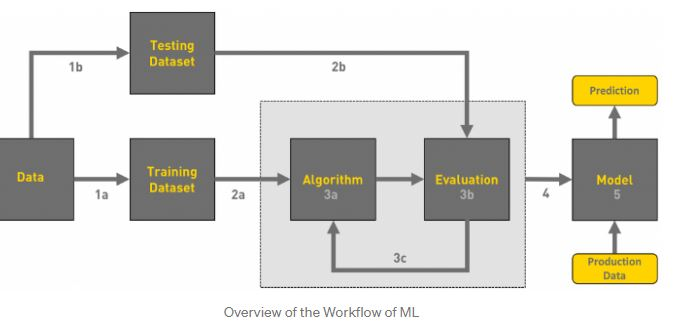
\includegraphics[width=100mm]{schematic.jpg}
	\caption{Graphical representation of the projects steps described above}
\end{figure}


\end{document}